\documentclass[letterpaper,11pt]{article}
\oddsidemargin -1.0cm \textwidth 17.5cm

\usepackage[utf8]{inputenc}
\usepackage[activeacute,spanish, es-lcroman]{babel}
\decimalpoint
\usepackage{amsfonts,setspace}
\usepackage{amsmath}
\usepackage{amssymb, amsmath, amsthm}
\usepackage{comment}
\usepackage{float}
\usepackage{amssymb}
\usepackage{dsfont}
\usepackage{anysize}
\usepackage{multicol}
\usepackage{enumerate}
\usepackage{graphicx}
\usepackage[left=1.5cm,top=2cm,right=1.5cm, bottom=1.7cm]{geometry}
\setlength\headheight{1.5em} 
\usepackage{fancyhdr}
\usepackage{multicol}
\usepackage{hyperref}
\usepackage{wrapfig}
\usepackage{subcaption}
\usepackage{siunitx}
\usepackage{cancel}
\pagestyle{fancy}
\fancyhf{}
\renewcommand{\labelenumi}{\normalsize\bfseries P\arabic{enumi}.}
\renewcommand{\labelenumii}{\normalsize\bfseries (\alph{enumii})}
\renewcommand{\labelenumiii}{\normalsize\bfseries \roman{enumiii})}


\begin{document}

\fancyhead[L]{\itshape{Facultad de Ciencias F\'isicas y Matem\'aticas}}
\fancyhead[R]{\itshape{Universidad de Chile}}

\begin{minipage}{11.5cm}
    \begin{flushleft}
        \hspace*{-0.6cm}\textbf{FI1000-6 Introducción a la Física Clásica}\\
        \hspace*{-0.6cm}\textbf{Profesora:} Paulina Lira\\
        \hspace*{-0.6cm}\textbf{Auxiliares:} Juan Cristóbal Castro \& Alejandro Silva\\
        \hspace*{-0.6cm}\textbf{Ayudantes:} Francisca Bórquez, Catalina Molina \& Erick Pérez\\
        
    \end{flushleft}
\end{minipage}

\begin{picture}(2,3)
    \put(366, 10){
\includegraphics[scale=0.9]{2020-1/Imágenes/logo/dfi-fcfm.pdf}}
\end{picture}

\begin{center}
	\LARGE\textbf{Auxiliar  \#3: MCU}\\
\end{center}

\vspace{-1cm}
\begin{enumerate}\setlength{\itemsep}{0.4cm}

\rfoot[]{pág. \thepage}

\item[]

\item Un mono se encuentra colgado de una rueda que gira horizontalmente con un periodo T, y que está a una altura H, como se indica en la figura. Además el eje sobre el cual gira la rueda esta en el borde de un plano inclinado, de ángulo $\theta$ con la horizontal. El mono se suelta justo cuando va pasando sobre el borde del plano inclinado tal que cae a una distancia D de ese punto. Determine el radio de la rueda
\begin{figure}[h!]
        \centering
        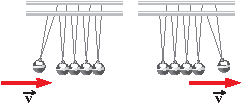
\includegraphics[scale=0.4]{2020-1/Imágenes/aux5/fig1.pdf}/
\end{figure}
    
    \item Considere un eje vertical de largo $L$, en cuyos extremos hay dos discos sólidos provistos de ranuras. Las ranuras están desplazadas un cierto ángulo $\theta$ entre sí. El sistema gira con una velocidad angular $\omega$ constante. Calcule la altura $H$ por sobre el disco superior, desde la cual se debe soltar una bolita para que esta, en caída libre, pase por ambas ranuras.

\begin{figure}[h!]
    \centering
    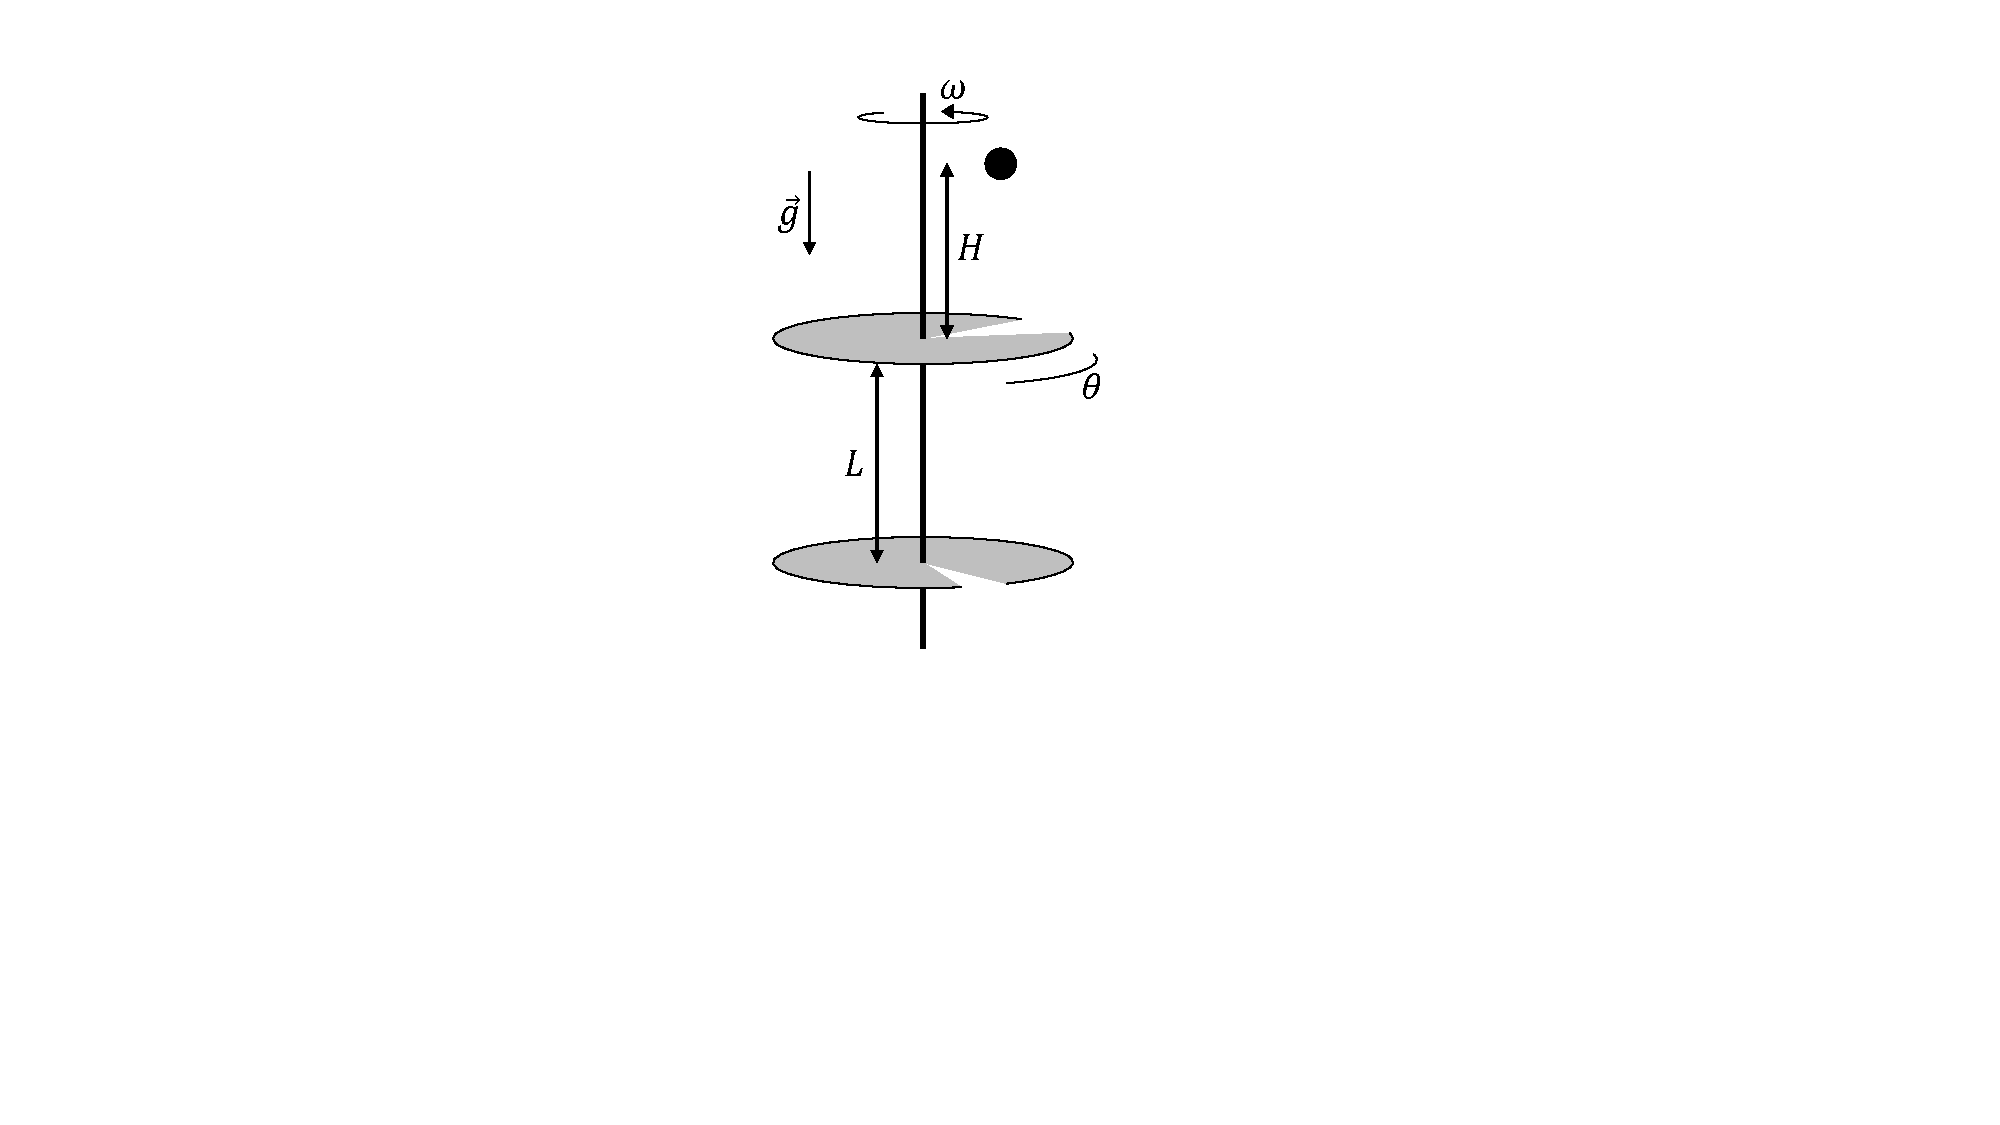
\includegraphics[scale=0.3]{2020-1/Imágenes/aux4/vara_pelota.pdf}
\end{figure}

\end{enumerate}
\end{document}